\begin{figure}
  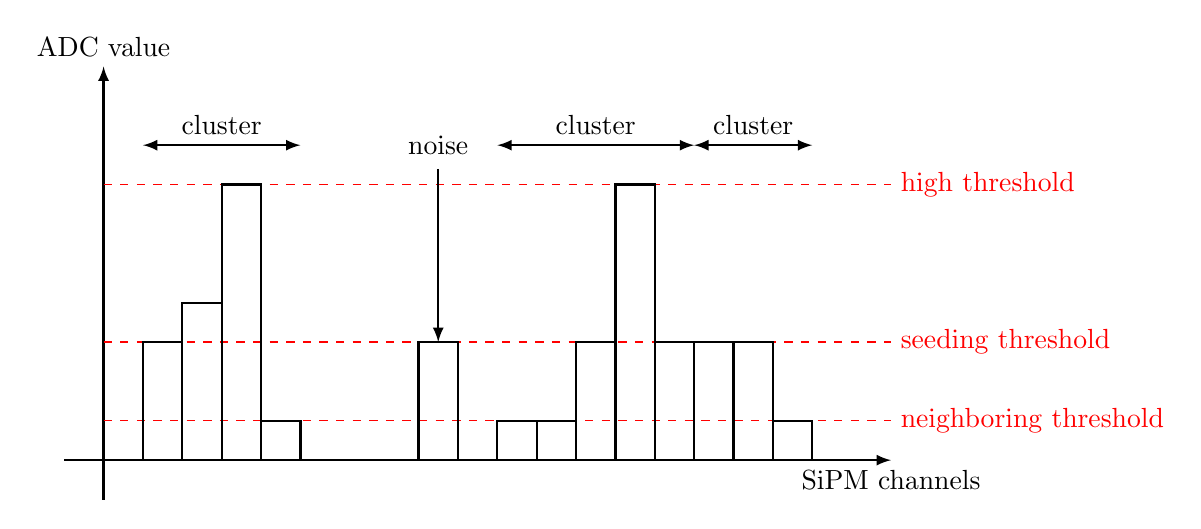
\begin{tikzpicture}
    % coordinates
    \draw[thick, black, -latex] (-0.5, 0) -- (10, 0) node [below] {SiPM channels};
    \draw[thick, black, -latex] (0, -0.5) -- (0, 5) node [above] {ADC value};
    % red lines
    \draw[dashed, red] (0, 0.5) -- (10, 0.5) node [above, right] {neighboring threshold};
    \draw[dashed, red] (0, 1.5) -- (10, 1.5) node [above, right] {seeding threshold};
    \draw[dashed, red] (0, 3.5) -- (10, 3.5) node [above, right] {high threshold};
    % clusters
    \draw[thick, black] (0.5, 0) -- (0.5, 1.5) -- (1, 1.5) -- (1, 0);
    \draw[thick, black] (1, 0) -- (1, 2) -- (1.5, 2) -- (1.5, 0);
    \draw[thick, black] (1.5, 0) -- (1.5, 3.5) -- (2, 3.5) -- (2, 0);
    \draw[thick, black] (2, 0) -- (2, 0.5) -- (2.5, 0.5) -- (2.5, 0);

    \draw[thick, black] (4, 0) -- (4, 1.5) -- (4.5, 1.5) -- (4.5, 0);

    \draw[thick, black] (5, 0) -- (5, 0.5) -- (5.5, 0.5) -- (5.5, 0);
    \draw[thick, black] (11/2, 0) -- (11/2, 1/2) -- (12/2, 1/2) -- (12/2, 0);
    \draw[thick, black] (12/2, 0) -- (12/2, 3/2) -- (13/2, 3/2) -- (13/2, 0);
    \draw[thick, black] (13/2, 0) -- (13/2, 7/2) -- (14/2, 7/2) -- (14/2, 0);
    \draw[thick, black] (14/2, 0) -- (14/2, 3/2) -- (15/2, 3/2) -- (15/2, 0);
    \draw[thick, black] (15/2, 0) -- (15/2, 3/2) -- (16/2, 3/2) -- (16/2, 0);
    \draw[thick, black] (16/2, 0) -- (16/2, 3/2) -- (17/2, 3/2) -- (17/2, 0);
    \draw[thick, black] (17/2, 0) -- (17/2, 1/2) -- (18/2, 1/2) -- (18/2, 0);

    % draw node cluster 1
    \draw[thick, black, latex-latex] (0.5, 4) -- (2.5, 4) node [above, midway] {cluster};

    % draw node cluster 2
    \draw[thick, black, -latex] (8.5/2, 3.7) -- (8.5/2, 1.5);
    \draw (8.5/2, 4) node {noise};

    % draw node cluster 3.1
    \draw[thick, black, latex-latex] (5, 4) -- (7.5, 4) node [above, midway] {cluster};

    % draw node cluster 3.1
    \draw[thick, black, latex-latex] (7.5, 4) -- (9, 4) node [above, midway] {cluster};
  \end{tikzpicture}
  \caption{Clusters are created by a group of channels from which one must be above the seeding threshold and the other channels being above the neighboring threshold. The other option is for one cluster being above the high threshold. Cluster with a width larger than four channels.}
  \label{fig:tikz_cluster}
\end{figure}
